% Options for packages loaded elsewhere
\PassOptionsToPackage{unicode}{hyperref}
\PassOptionsToPackage{hyphens}{url}
%
\documentclass[
  ignorenonframetext,
]{beamer}
\usepackage{pgfpages}
\setbeamertemplate{caption}[numbered]
\setbeamertemplate{caption label separator}{: }
\setbeamercolor{caption name}{fg=normal text.fg}
\beamertemplatenavigationsymbolsempty
% Prevent slide breaks in the middle of a paragraph
\widowpenalties 1 10000
\raggedbottom
\setbeamertemplate{part page}{
  \centering
  \begin{beamercolorbox}[sep=16pt,center]{part title}
    \usebeamerfont{part title}\insertpart\par
  \end{beamercolorbox}
}
\setbeamertemplate{section page}{
  \centering
  \begin{beamercolorbox}[sep=12pt,center]{part title}
    \usebeamerfont{section title}\insertsection\par
  \end{beamercolorbox}
}
\setbeamertemplate{subsection page}{
  \centering
  \begin{beamercolorbox}[sep=8pt,center]{part title}
    \usebeamerfont{subsection title}\insertsubsection\par
  \end{beamercolorbox}
}
\AtBeginPart{
  \frame{\partpage}
}
\AtBeginSection{
  \ifbibliography
  \else
    \frame{\sectionpage}
  \fi
}
\AtBeginSubsection{
  \frame{\subsectionpage}
}
\usepackage{lmodern}
\usepackage{amssymb,amsmath}
\usepackage{ifxetex,ifluatex}
\ifnum 0\ifxetex 1\fi\ifluatex 1\fi=0 % if pdftex
  \usepackage[T1]{fontenc}
  \usepackage[utf8]{inputenc}
  \usepackage{textcomp} % provide euro and other symbols
\else % if luatex or xetex
  \usepackage{unicode-math}
  \defaultfontfeatures{Scale=MatchLowercase}
  \defaultfontfeatures[\rmfamily]{Ligatures=TeX,Scale=1}
\fi
\usefonttheme{professionalfonts}
% Use upquote if available, for straight quotes in verbatim environments
\IfFileExists{upquote.sty}{\usepackage{upquote}}{}
\IfFileExists{microtype.sty}{% use microtype if available
  \usepackage[]{microtype}
  \UseMicrotypeSet[protrusion]{basicmath} % disable protrusion for tt fonts
}{}
\makeatletter
\@ifundefined{KOMAClassName}{% if non-KOMA class
  \IfFileExists{parskip.sty}{%
    \usepackage{parskip}
  }{% else
    \setlength{\parindent}{0pt}
    \setlength{\parskip}{6pt plus 2pt minus 1pt}}
}{% if KOMA class
  \KOMAoptions{parskip=half}}
\makeatother
\usepackage{xcolor}
\IfFileExists{xurl.sty}{\usepackage{xurl}}{} % add URL line breaks if available
\IfFileExists{bookmark.sty}{\usepackage{bookmark}}{\usepackage{hyperref}}
\hypersetup{
  pdftitle={Diseños de aliento y cumplimiento imperfecto},
  hidelinks,
  pdfcreator={LaTeX via pandoc}}
\urlstyle{same} % disable monospaced font for URLs
\newif\ifbibliography
\usepackage{color}
\usepackage{fancyvrb}
\newcommand{\VerbBar}{|}
\newcommand{\VERB}{\Verb[commandchars=\\\{\}]}
\DefineVerbatimEnvironment{Highlighting}{Verbatim}{commandchars=\\\{\}}
% Add ',fontsize=\small' for more characters per line
\usepackage{framed}
\definecolor{shadecolor}{RGB}{248,248,248}
\newenvironment{Shaded}{\begin{snugshade}}{\end{snugshade}}
\newcommand{\AlertTok}[1]{\textcolor[rgb]{0.94,0.16,0.16}{#1}}
\newcommand{\AnnotationTok}[1]{\textcolor[rgb]{0.56,0.35,0.01}{\textbf{\textit{#1}}}}
\newcommand{\AttributeTok}[1]{\textcolor[rgb]{0.77,0.63,0.00}{#1}}
\newcommand{\BaseNTok}[1]{\textcolor[rgb]{0.00,0.00,0.81}{#1}}
\newcommand{\BuiltInTok}[1]{#1}
\newcommand{\CharTok}[1]{\textcolor[rgb]{0.31,0.60,0.02}{#1}}
\newcommand{\CommentTok}[1]{\textcolor[rgb]{0.56,0.35,0.01}{\textit{#1}}}
\newcommand{\CommentVarTok}[1]{\textcolor[rgb]{0.56,0.35,0.01}{\textbf{\textit{#1}}}}
\newcommand{\ConstantTok}[1]{\textcolor[rgb]{0.00,0.00,0.00}{#1}}
\newcommand{\ControlFlowTok}[1]{\textcolor[rgb]{0.13,0.29,0.53}{\textbf{#1}}}
\newcommand{\DataTypeTok}[1]{\textcolor[rgb]{0.13,0.29,0.53}{#1}}
\newcommand{\DecValTok}[1]{\textcolor[rgb]{0.00,0.00,0.81}{#1}}
\newcommand{\DocumentationTok}[1]{\textcolor[rgb]{0.56,0.35,0.01}{\textbf{\textit{#1}}}}
\newcommand{\ErrorTok}[1]{\textcolor[rgb]{0.64,0.00,0.00}{\textbf{#1}}}
\newcommand{\ExtensionTok}[1]{#1}
\newcommand{\FloatTok}[1]{\textcolor[rgb]{0.00,0.00,0.81}{#1}}
\newcommand{\FunctionTok}[1]{\textcolor[rgb]{0.00,0.00,0.00}{#1}}
\newcommand{\ImportTok}[1]{#1}
\newcommand{\InformationTok}[1]{\textcolor[rgb]{0.56,0.35,0.01}{\textbf{\textit{#1}}}}
\newcommand{\KeywordTok}[1]{\textcolor[rgb]{0.13,0.29,0.53}{\textbf{#1}}}
\newcommand{\NormalTok}[1]{#1}
\newcommand{\OperatorTok}[1]{\textcolor[rgb]{0.81,0.36,0.00}{\textbf{#1}}}
\newcommand{\OtherTok}[1]{\textcolor[rgb]{0.56,0.35,0.01}{#1}}
\newcommand{\PreprocessorTok}[1]{\textcolor[rgb]{0.56,0.35,0.01}{\textit{#1}}}
\newcommand{\RegionMarkerTok}[1]{#1}
\newcommand{\SpecialCharTok}[1]{\textcolor[rgb]{0.00,0.00,0.00}{#1}}
\newcommand{\SpecialStringTok}[1]{\textcolor[rgb]{0.31,0.60,0.02}{#1}}
\newcommand{\StringTok}[1]{\textcolor[rgb]{0.31,0.60,0.02}{#1}}
\newcommand{\VariableTok}[1]{\textcolor[rgb]{0.00,0.00,0.00}{#1}}
\newcommand{\VerbatimStringTok}[1]{\textcolor[rgb]{0.31,0.60,0.02}{#1}}
\newcommand{\WarningTok}[1]{\textcolor[rgb]{0.56,0.35,0.01}{\textbf{\textit{#1}}}}
\usepackage{longtable,booktabs}
\usepackage{caption}
% Make caption package work with longtable
\makeatletter
\def\fnum@table{\tablename~\thetable}
\makeatother
\usepackage{graphicx}
\makeatletter
\def\maxwidth{\ifdim\Gin@nat@width>\linewidth\linewidth\else\Gin@nat@width\fi}
\def\maxheight{\ifdim\Gin@nat@height>\textheight\textheight\else\Gin@nat@height\fi}
\makeatother
% Scale images if necessary, so that they will not overflow the page
% margins by default, and it is still possible to overwrite the defaults
% using explicit options in \includegraphics[width, height, ...]{}
\setkeys{Gin}{width=\maxwidth,height=\maxheight,keepaspectratio}
% Set default figure placement to htbp
\makeatletter
\def\fps@figure{htbp}
\makeatother
\setlength{\emergencystretch}{3em} % prevent overfull lines
\providecommand{\tightlist}{%
  \setlength{\itemsep}{0pt}\setlength{\parskip}{0pt}}
\setcounter{secnumdepth}{-\maxdimen} % remove section numbering
% \usetheme{metropolis}  
\usepackage{fancyhdr}
\usepackage{lastpage}
\setbeamertemplate{footline}[frame number]{}
\setbeamertemplate{navigation symbols}{}
\pagenumbering{arabic}
% \usepackage[mathbf,mathcal]{euler}
\usepackage{multicol}


\newenvironment{cols}[1][]{}{}

\newenvironment{col}[1]{\begin{minipage}{#1}\ignorespaces}{%
\end{minipage}
\ifhmode\unskip\fi
\aftergroup\useignorespacesandallpars}

\def\useignorespacesandallpars#1\ignorespaces\fi{%
#1\fi\ignorespacesandallpars}

\makeatletter
\def\ignorespacesandallpars{%
  \@ifnextchar\par
    {\expandafter\ignorespacesandallpars\@gobble}%
    {}%
}
\makeatother

\title{Diseños de aliento y cumplimiento imperfecto}
\author{Diseño e implementación de experimentos en ciencias sociales\\
\emph{Departamento de Economía (UdelaR)}}
\date{}

\begin{document}
\frame{\titlepage}

\begin{frame}{Tipos de cumplimiento}
\protect\hypertarget{tipos-de-cumplimiento}{}
\begin{longtable}[]{@{}lll@{}}
\toprule
type & Treatment & Control\tabularnewline
\midrule
\endhead
Always-takers & Treated & Treated\tabularnewline
Compliers & Treated & Not Treated\tabularnewline
Never-takers & Not Treated & Not Treated\tabularnewline
Defiers & Not Treated & Treated\tabularnewline
\bottomrule
\end{longtable}
\end{frame}

\begin{frame}{Incumplimiento y resultados potenciales del tratamiento}
\protect\hypertarget{incumplimiento-y-resultados-potenciales-del-tratamiento}{}
\center 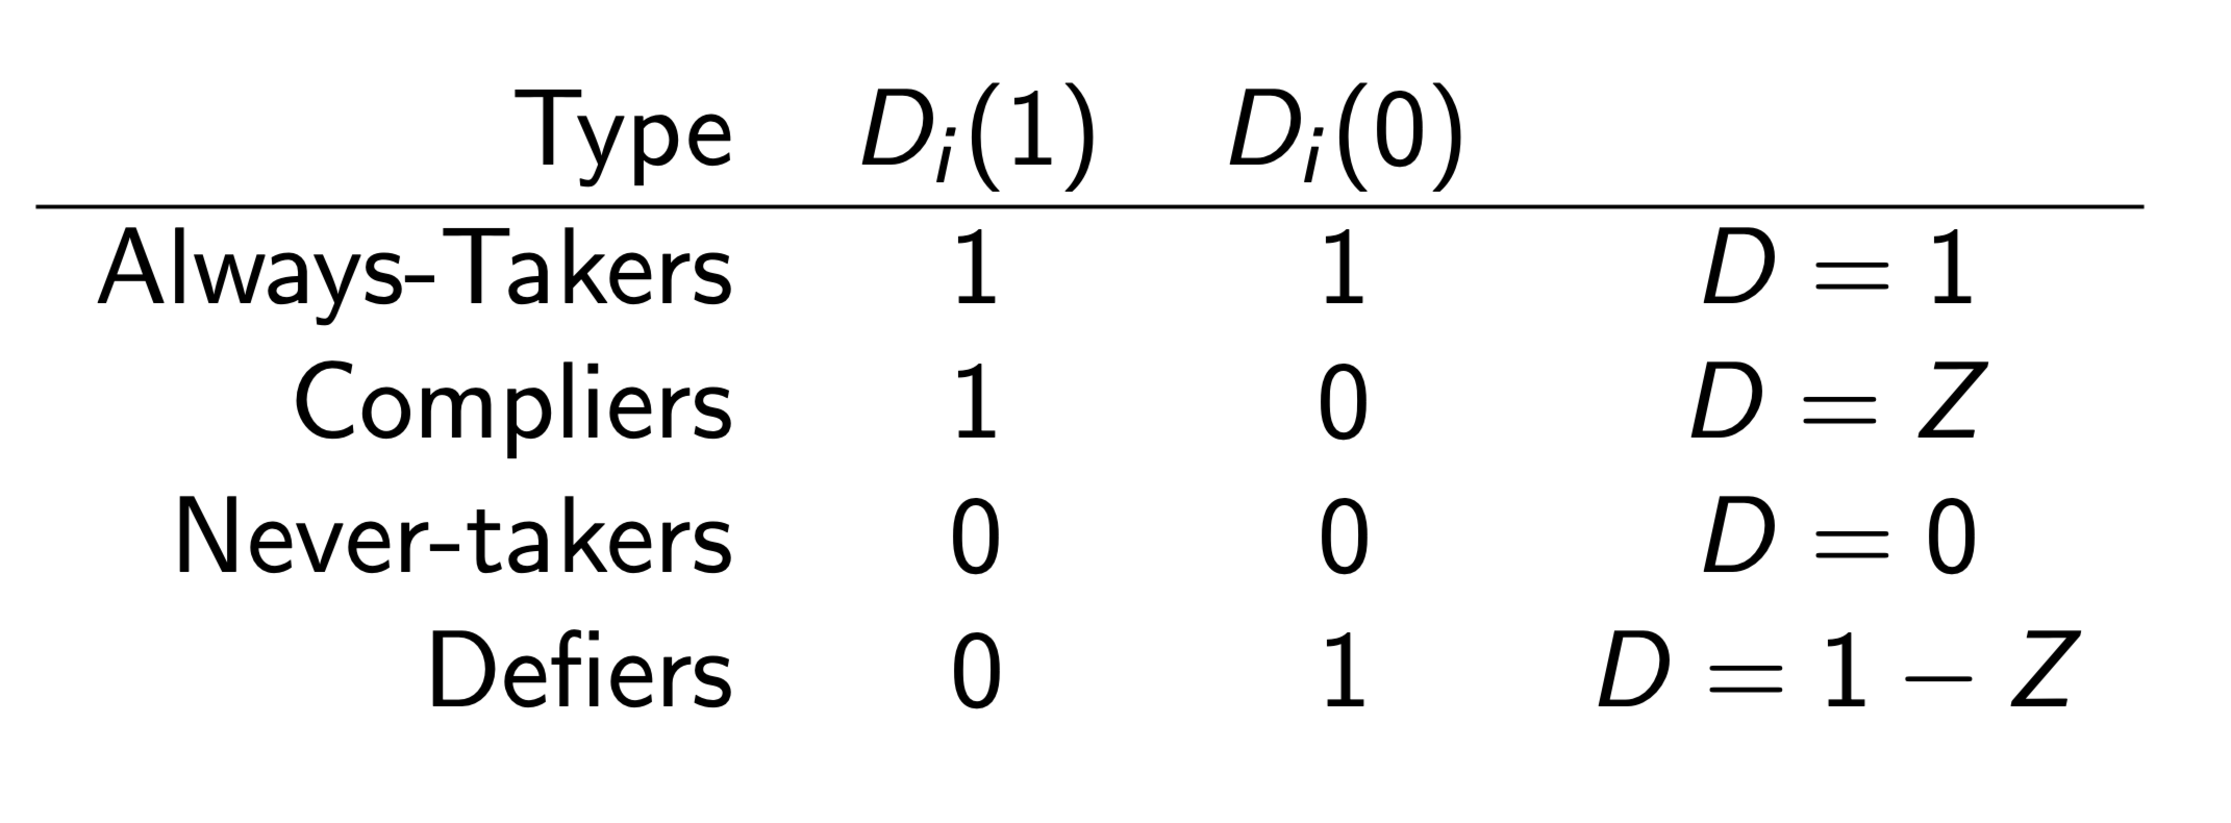
\includegraphics[width=0.8\textwidth,height=\textheight]{figs/one_sided}
\end{frame}

\begin{frame}{Tipos de efectos causales}
\protect\hypertarget{tipos-de-efectos-causales}{}
\begin{itemize}[<+->]
\tightlist
\item
  ITT: intención de tratar (\emph{intent to treat})
\item
  LATE: efecto local (\emph{local average treatment effect})

  \begin{itemize}[<+->]
  \tightlist
  \item
    También conocido como ``Complier Average Causal Effect'' (CACE).
  \end{itemize}
\end{itemize}
\end{frame}

\begin{frame}{Incumplimiento de un solo lado (one-sided noncompliance)}
\protect\hypertarget{incumplimiento-de-un-solo-lado-one-sided-noncompliance}{}
\center 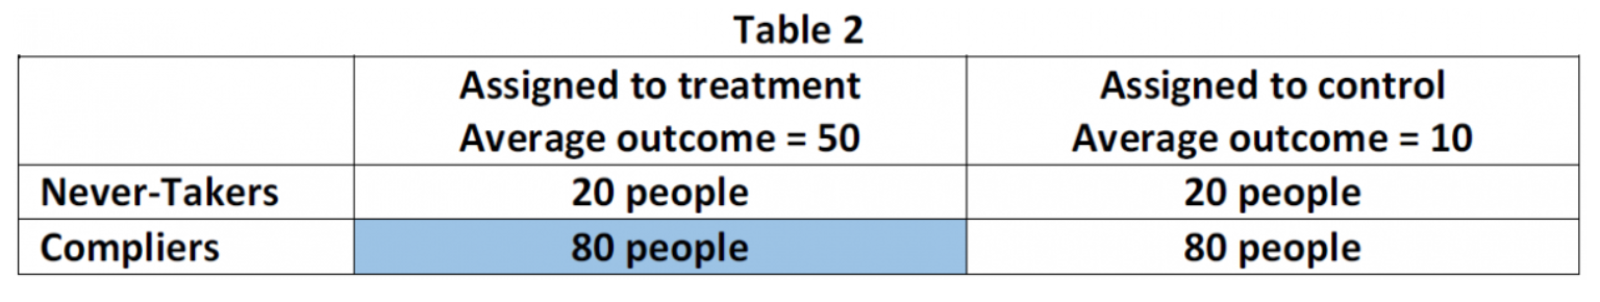
\includegraphics[width=1\textwidth,height=\textheight]{figs/compliers}

\begin{itemize}
\tightlist
\item
  100 son asignados aleatoriamente al tratamiento \pause 
\item
  80 son realmente tratados
\end{itemize}
\end{frame}

\begin{frame}{Incumplimiento de un solo lado (one-sided noncompliance)}
\protect\hypertarget{incumplimiento-de-un-solo-lado-one-sided-noncompliance-1}{}
\center

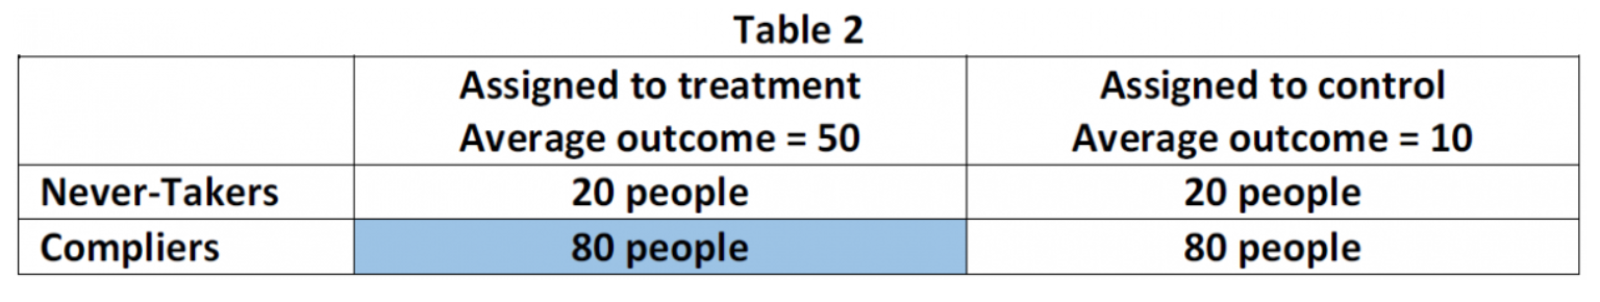
\includegraphics[width=1\textwidth,height=\textheight]{figs/compliers}

\begin{itemize}
\tightlist
\item
  Dado que \textcolor{violet}{la asignación es aleatoria} y sabemos que
  hay un 20\% de nunca-cumplidores (Never-Takers) en el grupo de
  tratamiento (columna de la izquierda),
  \textcolor{violet}{probablemente haya un 20\% de nunca-cumplidores en el grupo de control}.
  \pause
\item
  Dada la restricción de exclusión, los nunca-cumplidores tienen el
  mismo resultado potencial bajo las dos condiciones de tratamiento.
\end{itemize}
\end{frame}

\begin{frame}{Incumplimiento de un solo lado (one-sided)}
\protect\hypertarget{incumplimiento-de-un-solo-lado-one-sided}{}
\center 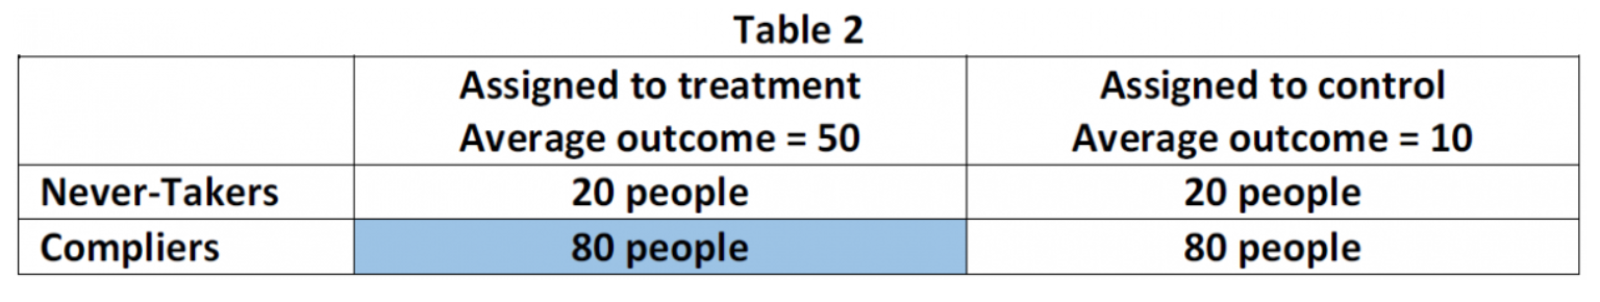
\includegraphics[width=1\textwidth,height=\textheight]{figs/compliers}

\begin{itemize}
\tightlist
\item
  La diferencia en los resultados medios (40) no puede atribuirse a los
  \emph{Never-takers}.
\item
  Por tanto, podemos atribuir todo el efecto ITT a los cumplidores.
\item
  El LATE puede calcularse dividiendo la estimación del ITT por la
  proporción de cumplidores:
\end{itemize}

\[40/0.8 = 50\]
\end{frame}

\begin{frame}{Incumplimiento de ambos lados (two-sided noncompliance)}
\protect\hypertarget{incumplimiento-de-ambos-lados-two-sided-noncompliance}{}
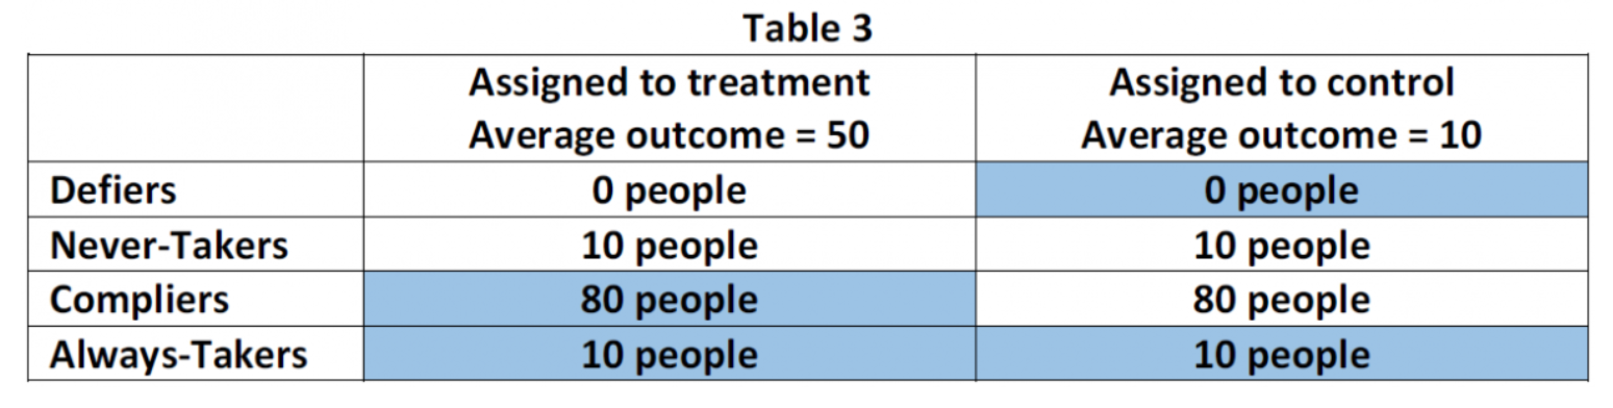
\includegraphics[width=1\textwidth,height=\textheight]{figs/compliers2}

Supuestos necesarios para estimar un LATE:

\begin{itemize}
\tightlist
\item
  Restricción de exclusión \pause
\item
  Que la población no contenga desfiantes (\emph{defiers}) (también
  denominado supuesto de ``monotonicidad'')
\end{itemize}
\end{frame}

\begin{frame}{Incumplimiento de ambos lados (two-sided noncompliance)}
\protect\hypertarget{incumplimiento-de-ambos-lados-two-sided-noncompliance-1}{}
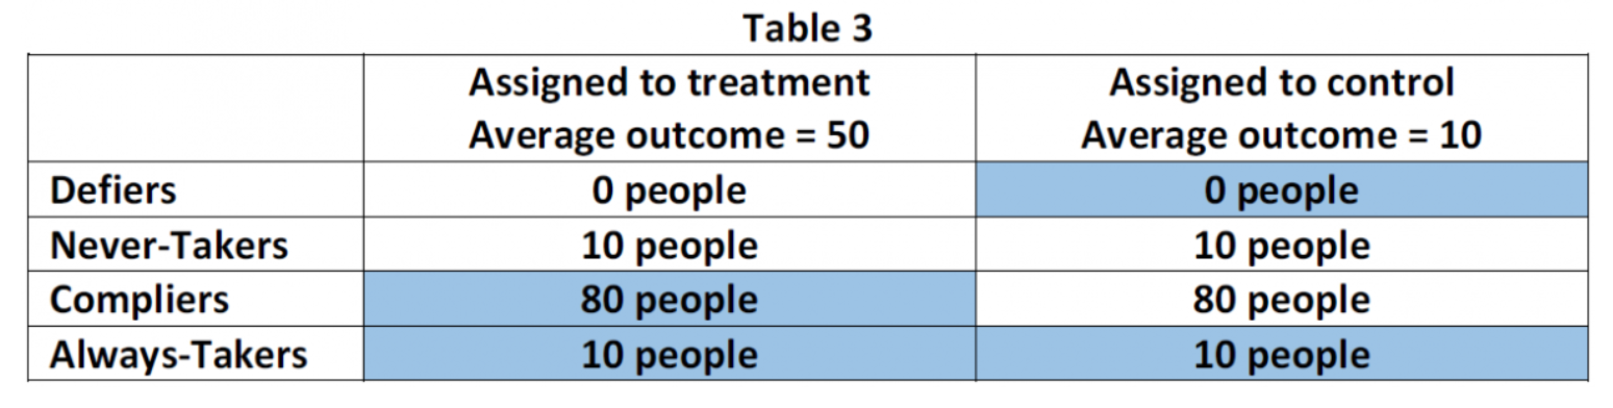
\includegraphics[width=1\textwidth,height=\textheight]{figs/compliers2}

\begin{itemize}
\item
  Podemos estimar el porcentaje de cumplidores: 100\% - 10\% (nunca
  cumplen) - 10\% (siempre cumplen) = 80\%.
\item
  LATE:
\end{itemize}

\[40/0.8 = 50\]
\end{frame}

\begin{frame}{LATE y variables instrumentales}
\protect\hypertarget{late-y-variables-instrumentales}{}
\[LATE = ATE_{complier} = ITT / ATE \text{ de Z en D}\]

\begin{itemize}
\item
  LATE es equivalente a una estimación por variables instrumentales.
\item
  Supongamos que 50 individuos de una población de 100 son asignados
  aleatoriamente al tratamiento.\pause 
\item
  La regresión (D\textasciitilde Z) da la proporción estimada de
  cumplidores: 80\%.
\item
  El efecto ITT: Y\textasciitilde Z. \pause
\item
  El LATE se calcula dividiendo por la proporción de cumplidores. \pause
\item
  El mismo resultados surge de una regresión MCO en dos etapas (2SLS) en
  la que el resultado (Y) se regresa sobre el tratamiento (D),
  utilizando la asignación al tratamiento como variable instrumental
  (Z).
\end{itemize}
\end{frame}

\begin{frame}[fragile]{LATE y variables instrumentales}
\protect\hypertarget{late-y-variables-instrumentales-1}{}
\[LATE = \frac{EffectZonY}{EffectZonD} = \frac{E[Y_i|Z_i=1]-E[Y_i|Z_i=0]}{E[D_i|Z_i=1]-E[D_i|Z_i=0]}\]
\pause

\tiny

\begin{Shaded}
\begin{Highlighting}[]
\NormalTok{Z \textless{}{-}}\StringTok{ }\KeywordTok{rep}\NormalTok{(}\DecValTok{0}\OperatorTok{:}\DecValTok{1}\NormalTok{,}\DecValTok{50}\NormalTok{) }\CommentTok{\# Assign 50 to treatment group (Z = 1), 50 to control group (Z = 0)}

\NormalTok{D \textless{}{-}}\StringTok{ }\NormalTok{Z           }\CommentTok{\# Compliers have D (treatment received) = Z (treatment assignment)}
\NormalTok{D[}\DecValTok{1}\OperatorTok{:}\DecValTok{10}\NormalTok{]  \textless{}{-}}\StringTok{ }\DecValTok{0}    \CommentTok{\# 10 Never Takers}
\NormalTok{D[}\DecValTok{11}\OperatorTok{:}\DecValTok{20}\NormalTok{] \textless{}{-}}\StringTok{ }\DecValTok{1}    \CommentTok{\# 10 Always Takers}

\NormalTok{Y        \textless{}{-}}\StringTok{ }\DecValTok{50}\OperatorTok{*}\NormalTok{D }\CommentTok{\# Compliers have Y = 50 if treated, 0 if not treated}
\NormalTok{Y[}\DecValTok{1}\OperatorTok{:}\DecValTok{10}\NormalTok{]  \textless{}{-}}\StringTok{ }\DecValTok{100}  \CommentTok{\# Never takers have high Y}
\NormalTok{Y[}\DecValTok{11}\OperatorTok{:}\DecValTok{20}\NormalTok{] \textless{}{-}}\StringTok{ }\DecValTok{0}    \CommentTok{\# Always takers have low Y}


\CommentTok{\# Estimated share of compliers }
\NormalTok{ITTD \textless{}{-}}\StringTok{ }\KeywordTok{coef}\NormalTok{(}\KeywordTok{lm}\NormalTok{(D}\OperatorTok{\textasciitilde{}}\NormalTok{Z))[}\DecValTok{2}\NormalTok{] }

\CommentTok{\# Estimated intention{-}to{-}treat effect}
\NormalTok{ITT  \textless{}{-}}\StringTok{ }\KeywordTok{coef}\NormalTok{(}\KeywordTok{lm}\NormalTok{(Y}\OperatorTok{\textasciitilde{}}\NormalTok{Z))[}\DecValTok{2}\NormalTok{] }

\CommentTok{\# LATE estimate}
\NormalTok{LATE \textless{}{-}}\StringTok{ }\NormalTok{ITT }\OperatorTok{/}\StringTok{ }\NormalTok{ITTD}

\KeywordTok{cbind}\NormalTok{(}\DataTypeTok{Y\_1 =} \KeywordTok{mean}\NormalTok{(Y[Z}\OperatorTok{==}\DecValTok{1}\NormalTok{]), }\DataTypeTok{Y\_0=}\KeywordTok{mean}\NormalTok{(Y[Z}\OperatorTok{==}\DecValTok{0}\NormalTok{]), ITTD, ITT, LATE)}
\end{Highlighting}
\end{Shaded}

\begin{verbatim}
##   Y_1 Y_0 ITTD ITT LATE
## Z  50  10  0.8  40   50
\end{verbatim}
\end{frame}

\begin{frame}[fragile]{LATE y variables instrumentales}
\protect\hypertarget{late-y-variables-instrumentales-2}{}
\tiny

\begin{Shaded}
\begin{Highlighting}[]
\CommentTok{\# install.packages(AER)}
\KeywordTok{summary}\NormalTok{(}\KeywordTok{ivreg}\NormalTok{(Y}\OperatorTok{\textasciitilde{}}\StringTok{ }\NormalTok{D }\OperatorTok{|}\StringTok{ }\NormalTok{Z)) }
\end{Highlighting}
\end{Shaded}

\begin{verbatim}
## 
## Call:
## ivreg(formula = Y ~ D | Z)
## 
## Residuals:
##    Min     1Q Median     3Q    Max 
##    -55     -5     -5     -5     95 
## 
## Coefficients:
##             Estimate Std. Error t value Pr(>|t|)    
## (Intercept)    5.000      5.660   0.883    0.379    
## D             50.000      8.839   5.657 1.53e-07 ***
## ---
## Signif. codes:  0 '***' 0.001 '**' 0.01 '*' 0.05 '.' 0.1 ' ' 1
## 
## Residual standard error: 35.36 on 98 degrees of freedom
## Multiple R-Squared: -0.1136, Adjusted R-squared: -0.125 
## Wald test:    32 on 1 and 98 DF,  p-value: 1.528e-07
\end{verbatim}
\end{frame}

\begin{frame}{Discusión}
\protect\hypertarget{discusiuxf3n}{}
\begin{itemize}
\tightlist
\item
  El LATE sólo refleja los efectos del tratamiento entre los
  cumplidores. \pause
\item
  La estimación LATE siempre es mayor que la estimación ITT. \pause
\item
  El LATE es un estimando importante en los diseños de ``aliento'' y en
  los ``downstream experiments''. \pause
\item
  Se puede utilizar un diseño con placebo para identificar el LATE (
  Gerber, Green, Kaplan, y Kern, 2010)
\end{itemize}
\end{frame}

\end{document}
